\chapter{Patterning in Synthetic Bacterial Colonies} \label{chapter3}
In chapter one we learned that systems might be more robust for patterning than linear stability analysis predicts and that we should look for other solutions.
We also learned that growth and boundaries might change the outcome too.

In chapter 2 we studied the patterning capabilities of this new gene circuit. we showed it could make patterns. We also identified certain parameter regimes which are more robust for patterning. For example, matching transfer functions or adding aTc,DAPG or slowing $D_{V}$ diffusion.
Finally, in chapter 2 we parametrised the model under liquid culture experiments which have followed the circuit tuning guidance to optimise Turing robustness.

Following chapter 2 insights, I carried out spatial experiments were carried out with the optimal tuning conditions.
In this chapter, we combine both chapter 1 and 2 knowledge and apply those spatial experiments based on our previous work.
The aim is to predict pattern formation under the chosen spatial setup which are growing colonies.
Additionally, for the patterns obtain, the aim is to obtain mechanistic insights of what the patterns can do.
This is done first with the general parameter distribution from the literature to explore the overall potential of the circuit in bacterial colonies.
Then, is done in the parametrised distributions to get more specific insights into the mechanisms in the regions we find ourselves in and to have a more predictable model.

\section{Rings in small colonies with high aTc}
In the previous chapter, we found certain conditions which could affect robustness for Turing pattern formation.
As already shown, the circuit components were matched by Jure Tica and Tong Zhu (see Fig~\ref{fig:dose_response_experimental}) to improve robustness as seen in Fig.~\ref{fig:balancing_robustness}.
In this section, I investigate the circuit in a biofilm using confocal microscopy under those optimal Turing conditions.
More specifically, I look at how the biofilm fluourescent patterns change with different levels of aTc.

MK01 \textit{E.coli} cells were transformed using electroporation (Section~\ref{electroporation}) with the full circuit.
This involved the introduction of 4 plasmids with the three nodes and the regulator cassette as seen in Fig.~\ref{fig:synthetic circuit_chapter2} and Table~\ref{tab:plasmid table} into our \textit{E.coli} cells.
For this, the cells were then plated in 6 well MatTek plates and grew as individual colonies which are radially growing biofilms.
These growing colonies are then imaged using confocal microscopy.
Confocal microscopy is a type of fluorescence microscopy used to image thicker objects, where the beam of light focuses on one depth level, meaning you can get a single z plane of fluorescence.
This way we can obtain a 2D fluorescence pattern steaming from a single focal plane of the colony ~\parencite{semwogerere2005confocal}.
 Detailed methods on colony plating and microscopy can be found in Section~\ref{microscopy}
Red and green channels were imaged to detect mCherry and GFP as seen in Fig.~\ref{rgchannels}A,B.
These channels can then be superposed to get a GFP-mCherry combined reading (Fig.~\ref{rgchannels}C)
\begin{figure}[H]

    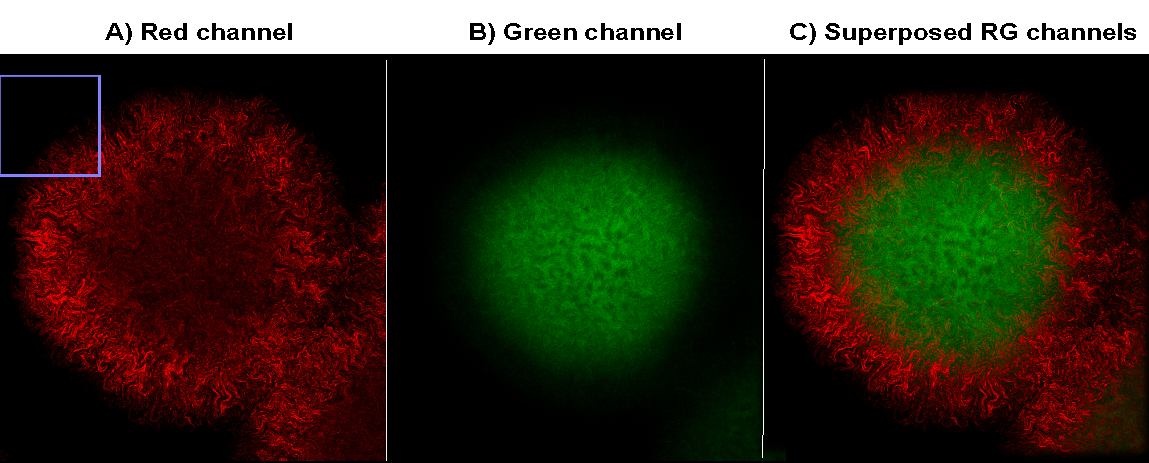
\includegraphics[width=1\textwidth]{chapters/Chapter 3/rgchannels}
    \caption{add}
    \label{rgchannels}
\end{figure}

To test the impact of aTc on the patterning of the circuit, we prepared the agar on the MaTek plates with different levels of aTc, ranging from 0 to $10^1 \mu M$.
Different colony patterns arise from this aTc walk as seen in Fig.~\ref{atcwalk_timeseries_confocal}A.
The colonies exhibiting more spatially heterogeneous behaviour are those with high aTc ($10^1 \mu M$).
This high aTc condition is further explored by imaging every day.
In Fig.~\ref{atcwalk_timeseries_confocal}B, we see how over time, the center of the colony oscillates from black to red to green.
As this happens, rings get added from the center as in~\cite{Konow2019}'s inner ring addition mechanism.
The final snapshot (64h) shows green, red, green, red progression steaming from the center.

\begin{figure}[H]

    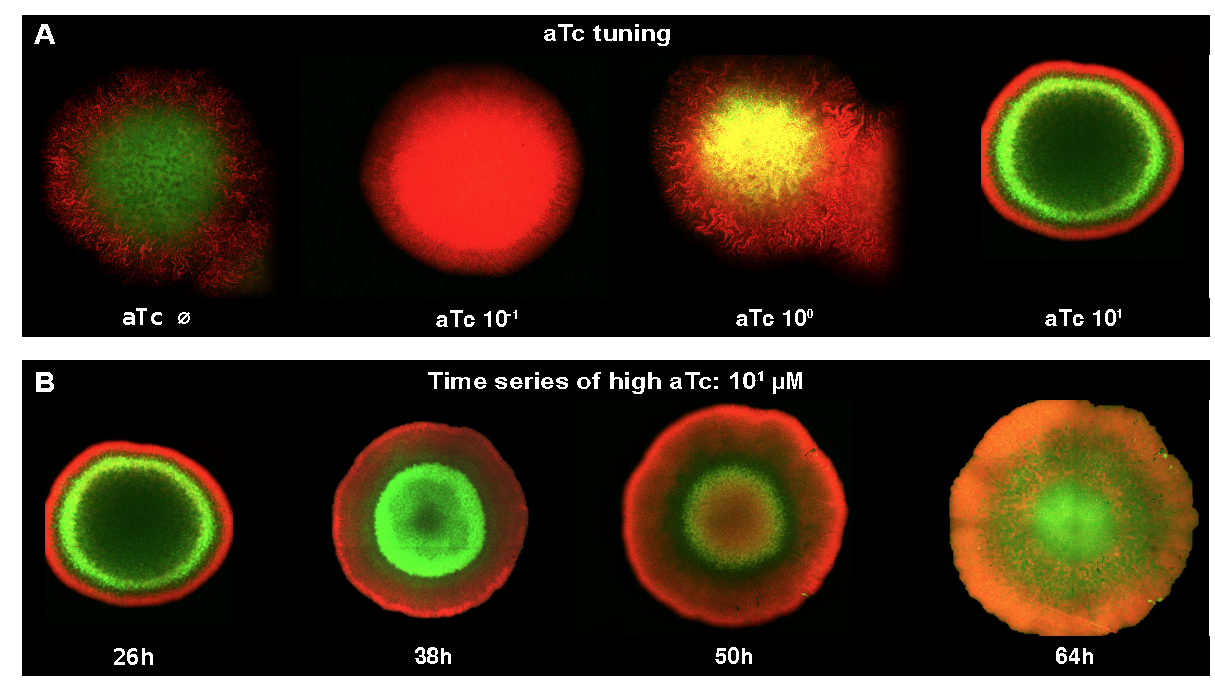
\includegraphics[width=1\textwidth]{chapters/Chapter 3/atcwalk_timeseries_confocal}
    \caption{\textbf{Confocal images of small colonies with gene circuit 3943}. A) Colonies with different atc conditions at time 26h: no aTc $10^{-1} \mu M,10^{0} \mu M,10^{1} \mu  $. B) Time series of single colony with high aTc condition ($10^1 \mu M$).}
    \label{atcwalk_timeseries_confocal}
\end{figure}




\section{Modelling synthetic circuit in tissues}

\subsection{shape}
\subsection{cellular automata}
\section{Explore patterning potential}
\subsection{general params}
\subsection{parametrised params}



%\section{Modelling bacterial colonies}
%\subsection{openboundary circle shape growth noise}
%\section{Explore patterning potential}
%\subsection{general params}
%\subsection{parametrised params}
